\documentclass[a4 paper, 12pt]{article}
\usepackage[utf8]{inputenc}

%% preamble
% preamble.tex

%% packages
% IEEE conference needed
\usepackage{times}
\usepackage{amssymb}
\usepackage{amsmath}
% \usepackage{mathptmx}               % comment for non-IEEE style
\usepackage{graphics}
\usepackage{epsfig}
% others
\usepackage{nicefrac}               % For nice fraction like 1/2
\usepackage{geometry}               % For setting layout
\usepackage{enumitem}               % For customizing items
% For tables
\usepackage{multirow}
\usepackage{makecell}
\usepackage{diagbox}

\usepackage{enumitem}

\usepackage{amsthm}

\usepackage{cite}



%% settings for normal a4 layout
% set indent
% \setlength{\parindent}{0pt}
\setlength{\parskip}{1em}
% set layout
% \geometry{a4paper,scale=0.8}
\geometry{a4paper,left=3cm,right=3cm,top=3cm,bottom=3cm}
% correct bad hyphenation here
\hyphenation{op-tical net-works semi-conduc-tor}


%% new commands
% text
\newcommand{\tn}[1]{\textnormal{#1}}
\newcommand{\tb}[1]{\textbf{#1}}
\newcommand{\ti}[1]{\textit{#1}}
% matrices
\newcommand{\mat}[0]{\begin{bmatrix}}
\newcommand{\mate}[0]{\end{bmatrix}}
% states
\newcommand{\vx}{\mathbf{x}}
\newcommand{\vp}{\mathbf{p}}
\newcommand{\vv}{\mathbf{v}}
\newcommand{\va}{\mathbf{a}}
\newcommand{\vb}{\mathbf{b}}
\newcommand{\vz}{\mathbf{z}}
\newcommand{\vd}{\mathbf{d}}
\newcommand{\vu}{\mathbf{u}}
\newcommand{\vf}{\mathbf{f}}
\newcommand{\vg}{\mathbf{g}}
\newcommand{\vh}{\mathbf{h}}
\newcommand{\vs}{\mathbf{s}}
% sets
\newcommand{\W}{\mathcal{W}}        % Workspace
\newcommand{\X}{\mathcal{X}}        % Configuration space
\newcommand{\Obs}{\mathcal{O}}      % Obstacle regions
\newcommand{\A}{\mathcal{A}}        % Robot occupied space
\newcommand{\U}{\mathcal{U}}        % Control space
\newcommand{\Z}{\mathcal{Z}}        % General decision variables space
\newcommand{\rN}{\mathcal{N}}       % Agent index sets
\newcommand{\oM}{\mathcal{M}}       % Dynamic obstacle index sets
% numbers set
\newcommand{\R}{\mathbb{R}}
\newcommand{\N}{\mathbb{N}}
% operator
\newcommand\norm[1]{\left\|#1\right\|}      % Big norm
\newcommand\abs[1]{\left|#1\right|}         % Big abs
\newcommand\inv[1]{#1^{-1}}                 % Inverse
\newcommand{\atwo}{\mathrm{atan2}}
\newcommand\mc[1]{\mathcal{#1}}
% statistics
\newcommand{\hx}{\hat{\mathbf{x}}}
\newcommand{\hp}{\hat{\mathbf{p}}}
\newcommand{\vsigma}{\mathbf{\sigma}}
\newcommand{\vomega}{\mathbf{\omega}}
\newcommand{\mN}{\mathcal{N}}
\newcommand{\pr}{\textnormal{Pr}}
% symbols
\newcommand{\eps}{\varepsilon}
% other
\newcommand{\ra}{\rightarrow}
\newcommand{\RA}{\Rightarrow}
\newcommand{\half}{\frac{1}{2}}
\newcommand{\quater}{\frac{1}{4}}


%% theorems
\newtheorem{rmk}{\textbf{Remark}}
\newtheorem{thm}{\textbf{Theorem}}
\newtheorem{prop}{\textbf{Proposition}}
\newtheorem{prob}{\textbf{Problem}}
\newtheorem{defi}{\textbf{Definition}}
\newtheorem{algo}{\textbf{Algorithm}}
\newtheorem{cons}{\textbf{Constraint}}


%% title information
\title{
        \Large{DISC Course: Multi-agent Network Dynamics and Games}\\
        \vspace{1em}
        \large\tb{Homework 3 \& 4}
}
\author{
        \small Hai Zhu                          \\
        \small Delft University of Technology   \\
        \tt\small h.zhu@tudelft.nl
 }
\date{\small\ti{\today}}

%% document
\begin{document}
%% title
\maketitle

\section{Homework 3}
~~~~
\tb{Problem 1}

\tb{Solution: }
\tb{a)} For different values of $x$,
\begin{itemize}
        \item Case 1: $x=0$. \\
        The payoff matrix is 
        \begin{center}
                \begin{tabular}{ | m{1em} | m{1em}| } 
                \hline
                1,1& 2,0 \\ 
                \hline
                0,2 & 3,3 \\ 
                \hline
                \end{tabular}
        \end{center}
        There are two pure strategy Nash equilibria: $(e_1,e_1)$ and $(e_2,e_2)$.

        Apparently, $(e_2,e_2)$ is a strict symmetric Nash equilibrium. Thus, $e_2$ is an evolutionary stable strategy (Corollary 5.53 in \cite{b1}). For $e_1$, since we have $\pi(e_1,e_1)>\pi(e_2,e_1)$, thus $e_1$ is also an evolutionary stable strategy.

        \item Case 2: $x=1$. \\
        The payoff matrix is 
        \begin{center}
                \begin{tabular}{ | m{1em} | m{1em}| } 
                \hline
                1,1& 2,1 \\ 
                \hline
                1,2 & 3,3 \\ 
                \hline
                \end{tabular}
        \end{center}
        There are two pure strategy Nash equilibria: $(e_1,e_1)$ and $(e_2,e_2)$.

        Similarly, since $(e_2,e_2)$ is a strict symmetric Nash equilibrium. Thus, $e_2$ is an evolutionary stable strategy (Corollary 5.53 in \cite{b1}). For $e_1$, we have $\pi(e_1,e_1)=\pi(e_2,e_1)$ but $\pi(e_1,e_2)<\pi(e_2,e_2)$. So $e_1$ is not an evolutionary stable strategy.

        \item Case 3: $x = 2$. \\
        The payoff matrix is 
        \begin{center}
                \begin{tabular}{ | m{1em} | m{1em}| } 
                \hline
                1,1& 2,2 \\ 
                \hline
                2,2 & 3,3 \\ 
                \hline
                \end{tabular}
        \end{center}
        There is only one pure strategy Nash equilibria: $(e_2,e_2)$. 

        Note that the only one pure strategy Nash equilibrium is strict symmetric. Thus $e_2$ is the evolutionary stable strategy (Corollary 5.53 in \cite{b1}). 

\end{itemize}

\tb{b)} Recall the definition of weakly dominated strategy \cite{b1}:
\begin{defi}
        A strategy $s_i$ of player $i$ is termed weakly dominated if there exists another strategy $t_i$ of player $i$ satisfying the following two conditions:\vspace{-0.5em}

        (i) For every strategy vector $s_{-i}$ of other players,
        \begin{equation}\label{eq:WD1}
                \pi(s_i,s_{-i}) \leq \pi(t_i,s_{-i})
        \end{equation}
        \vspace{-2.5em}

        (ii) There exists a strategy vector $t_{-i}$ of other players such that 
        \begin{equation}\label{eq:WD2}
                \pi(s_i,t_{-i}) < \pi(s_i,t_{-i})
        \end{equation}
\end{defi}
If the equal condition in equation (\ref{eq:WD1}) is removed, then the above definition is refined to ``strictly dominated''.

In the given game, since $X$ is weakly dominated and $(X,X)$ is a Nash equilibrium, we have 
\begin{align}
        & c = a \\
        & d > b
\end{align}
We can compute
\begin{equation}
        \pi(X,X) = a
\end{equation}
\begin{equation}
        \pi(Y,X) = c
\end{equation}
We further compute that 
\begin{equation}
        \pi(X,Y) = b
\end{equation}
\begin{equation}
        \pi(Y,Y) = d
\end{equation}
Thus we have $\pi(X,X) = \pi(Y,X)$ but $\pi(X,Y) < \pi(Y,Y)$. Hence, $X$ is not an evolutionary stable strategy.



\tb{Problem 2}

\tb{Solution:} \tb{a)} 
Let $s_1 = e_1$ the first pure strategy of player 1. We can suppose $t_i = e_2, e_3, e_4$ and check if it satisfies the above conditions. The result they all do not satisfy the conditions since 
\begin{equation}
        \begin{aligned}
                \pi(e_1,e_2) > \pi(e_2,e_2) \\
                \pi(e_1,e_1) > \pi(e_3,e_1) \\
                \pi(e_1,e_3) > \pi(e_4,e_3)
        \end{aligned}
\end{equation}
which contradicts with equation (\ref{eq:WD1}). Hence, the first pure strategy of player 1 is not dominated by a pure strategy.

\tb{b)} We suppose that it is weakly dominated by a mixed strategy $p = [p_1,p_2,p_3,p_4]^T$. Then the payoff of player 1 by choosing this mixed strategy is 
\begin{equation}
        \pi(p,q) = p^TAq
\end{equation}
where $q = [q_1,q_2,q_3,q_4]$ is a strategy of the other player. Then according to the definition of ``weakly dominated'', we can get the following condition
\begin{align}
        &p^TAq \geq e_1^TAq, \hspace{0.2cm} \forall q\in Q \\
        &p^TAq > e_1^Tq, \hspace{0.2cm} \exists q\in Q
\end{align}
where $Q$ is the strategy space of the other player. The above conditions can be written more clearly as follows
\begin{align}
        &[p_1,p_2,p_3,p_4]A \geq [1,2,0,-2] \\
        &\norm{[p_1,p_2,p_3,p_4]A} > \norm{[1,2,0,-2]} \\
        &p_1 + p_2 + p_3 + p_4 = 1
\end{align}
To solve the above underdetermined equation, we can use optimization based method such as linear programming. Here is a solution $p = [0, \frac{2}{3}, \frac{1}{3}, 0]^T$. Furthermore, we can valid that this mixed strategy actually strictly dominants the first pure strategy.

\tb{c)} Yes. We have shown that the mixed strategy $p = [0, \frac{2}{3}, \frac{1}{3}, 0]^T$ strictly dominants the first pure strategy in previous question.

\tb{d)} No, it is impossible. According to the Theorem 5.20 in \cite{b1}, in every Nash equilibrium of a game in strategic form, the pure strategy strictly dominated by a mixed strategy is chosen by the player with probability 0. Since we have shown that the first pure strategy of player 1 is strictly dominated by a mixed strategy, it is impossible that it is at a Nash equilibrium.

\tb{e)} Use the definition of strictly dominated, we can valid the following statements:
\begin{itemize}
        \item The first pure strategic $e_1$ of player 1 is strictly dominated by a mixed strategy $p = [0, \frac{2}{3}, \frac{1}{3}, 0]^T$.
        \item The forth pure strategic $e_4$ of player 1 is strictly dominated by a mixed strategy $p = [0, \frac{2}{3}, \frac{1}{3}, 0]^T$.
\end{itemize}
Therefore, the set of Nash equilibrium is confined to the space of strategies $e_2$ and $e_3$, esulting in the following two-player payoff table:
\begin{center}
        \begin{tabular}{ | m{1em} | m{1em}| } 
        \hline
        1,1& 1,4 \\ 
        \hline
        4,1 & 3,3 \\ 
        \hline
        \end{tabular}
\end{center}
It can be verified that 
\begin{align}
        \pi(e_3,e_3) > \pi(e_2,e_3) \label{eq:2.Na1} \\
        \pi(e_3,e_3) > \pi(e_3,e_2) \label{eq:2.Na2}
\end{align}
Hence, $(e_3,e_3)$ is a pure strategy Nash equilibrium of the symmetric game.

\tb{f)} According to the Theorem 5.51 in \cite{b1}, for any two-player symmetric game, an evolutionary stable equilibrium is also a Nash equilibrium. Since we have shown that there is only one Nash equilibrium $(e_3,e_3)$ of the given game in previous questions, we only need to check if it is evolutionary stable. 

Please observe equation (\ref{eq:2.Na1}) and (\ref{eq:2.Na2}). It shows that $(e_3,e_3)$ is a strict symmetric Nash equilibrium, then the conditions for ESS hold (Corollary 5.53 \cite{b1}). Hence, $e_3$ is an evolutionary stable strategy in this game.


\tb{Problem 3}
\begin{proof}

To show that ``can be'', I only need to give an example to support the statement. Consider the following payoff matrix
\begin{equation}
        \left[
        \begin{array}{ccc}
        0 & 1 & 0 \\
        0 & 0 & 2 \\
        0 & 0 & 1
        \end{array}
        \right]
\end{equation}
The replicator dynamics are
\begin{equation}
        \left[
        \begin{array}{c}
        \dot{x_1} \\
        \dot{x_2} \\
        \dot{x_3} 
        \end{array}
        \right]
        =
        \left[
        \begin{array}{c}
        -x_1(x_1x_2 - x_2 + x_3(2x_2 + x_3))\\
        -x_2(x_1x_2 - 2x_3 + x_3(2x_2 + x_3))\\
        -x_3(x_1x_2 - x_3 + x_3(x_2 + x_3))
        \end{array}
        \right]
\end{equation}
It can be verified that in this game, $(e_1,e_1)$ is the unique Nash equilibrium. However, $e_1$ is not Lyapunov stable. The proof is given below: Define a ball around $e^1$ with $r>0$ as $B_r=\{x\in \Delta | \hspace{0.5em}||x-e_1|| \le r\}$. Furthermore, let $V(x)=\frac{1}{2}^Tx$ be a Lyapunov function candidate. Then we have $\dot{V(x)}=x^T\dot{x}$. 

According to the Theorem 4.3 from  if $\forall x^* \in B_r$ if $\dot{V(x)}>0$ then $e^1$ is unstable. If we check for the neighbor mixed strategy of $e^1$ $x_{test}=[1-\epsilon \hspace{0.5em} \epsilon \hspace{0.5em}0]^T | \epsilon >0$ we get $\dot{V(x_{test})=
e^2*(2*e^2 - 3*e + 1)>0}$ with $\epsilon$ sufficiently small. This concludes the proof that a state can be a $\omega$-limit point without being stable.


\end{proof}


\tb{Problem 4}
\begin{proof}


For this theorem, there is a proof in \cite{b4} (Proposition 3.13).
        
% Recall the definition of asymptotically stable set (Theorem 6.3 \cite{b2}):
% \begin{defi}
%         Suppose that $A \in C$ is a closed set. Then $A$ is asymptotically stable if and only if there exists a neighborhood $D$ of $A$ and a continuous function $v:D\ra R_+$ satisfying the following conditions:
%         \begin{equation}
%                 v(x) = 0 \hspace{0.4cm} \tn{if and only if } x\in A,
%         \end{equation}
%         \begin{equation}
%                 v(\xi(t,x)) < v(x) \hspace{0.4cm} \tn{if } x\notin A, t>0, \tn{and } \xi(s,x)\in D ~~\forall s\in[0,t].
%         \end{equation}
% \end{defi}

\end{proof}


\section{Homework 4}
~~~~~
\tb{Problem 1}

\tb{Solution:}
\tb{a)} The replicator dynamics can be written as 
\begin{equation}
        \dot{x}=
        \left[
        \begin{array}{c}
         -x_1 (u x_3 - x_4 + x_1 x_2 + x_1 x_4 + x_2 x_3 + x_3 x_4 - 2 u x_1 x_3 - 2 u x_2 x_4)\\
         -x_2 (u x_4 - x_1 + x_1 x_2 + x_1 x_4 + x_2 x_3 + x_3 x_4 - 2 u x_1 x_3 - 2 u x_2 x_4)\\
         -x_3 (u x_1 - x_2 + x_1 x_2 + x_1 x_4 + x_2 x_3 + x_3 x_4 - 2 u x_1 x_3 - 2 u x_2 x_4)\\
         -x_4 (u x_2 - x_3 + x_1 x_2 + x_1 x_4 + x_2 x_3 + x_3 x_4 - 2 u x_1 x_3 - 2 u x_2 x_4)\\
        \end{array}
        \right]
\end{equation}
Let $\dot{x} = 0$ and then we can get the equilibrium points of the replicator dynamics:
\begin{center}
        \begin{tabular}{c c c c} 
        \hline
        $x_1$ & $x_2$ & $x_3$ & $x_4$ \\ 
        \hline
        $\frac{1}{2}$ & 0 & $\frac{1}{2}$ & 0\\ 
        % \hline
        0 & $\frac{1}{2}$ & 0 & $\frac{1}{2}$\\ 
        % \hline
        $\frac{1}{4}$ &  $\frac{1}{4}$ & $\frac{1}{4}$ &  $\frac{1}{4}$\\ 
        % \hline
        $\frac{\mu}{\mu^2 + 2 \mu - 1}$ & $\frac{\mu (\mu + 1)}{\mu^2 + 2 \mu - 1}$ & $\frac{-1}{\mu^2 + 2 \mu - 1}$ & 0\\ 
        % \hline
        $\frac{\mu (\mu + 1)}{\mu^2 + 2 \mu - 1}$  &  $\frac{-1}{\mu^2 + 2 \mu - 1}$ & 0 & $\frac{\mu}{\mu^2 + 2 \mu - 1}$\\ 
        % \hline
        0 & $\frac{\mu}{\mu^2 + 2\mu - 1}$ & $\frac{\mu (\mu + 1)}{\mu^2 + 2 \mu - 1}$ & $\frac{-1}{\mu^2 + 2\mu - 1}$\\ 
        % \hline
        $\frac{-1}{\mu^2 + 2\mu - 1}$ & 0 & $\frac{\mu}{\mu^2 + 2\mu - 1}$ & $\frac{\mu(\mu + 1)}{\mu^2 + 2\mu - 1}$\\ 
        \hline
        \end{tabular}
\end{center}

\tb{b)} According to the results of question a), the only interior equilibrium point is $[\frac{1}{4},~ \frac{1}{4},~ \frac{1}{4},~ \frac{1}{4}]$. Thus we can get its Jacobian matrix:
\begin{equation}
        J=\left[
        \begin{array}{cccc}
           \frac{\mu}{8} - \frac{1}{8} &   \frac{\mu}{8} - \frac{1}{8}& - \frac{\mu}{8} - \frac{1}{8}&   \frac{\mu}{8} + \frac{1}{8} \\
           \frac{\mu}{8} + \frac{1}{8}&   \frac{\mu}{8} - \frac{1}{8}&   \frac{\mu}{8} - \frac{1}{8}& - \frac{\mu}{8} - \frac{1}{8} \\
         - \frac{\mu}{8} - \frac{1}{8}&   \frac{\mu}{8} + \frac{1}{8}&   \frac{\mu}{8} - \frac{1}{8}&   \frac{\mu}{8} - \frac{1}{8} \\
           \frac{\mu}{8} - \frac{1}{8}& - \frac{\mu}{8} - \frac{1}{8}&   \frac{\mu}{8} + \frac{1}{8}&   \frac{\mu}{8} - \frac{1}{8} 
        \end{array}
        \right]
\end{equation}
The eigenvalues can be calculated then, which are $\lambda = \frac{\mu}{8} - \frac{1}{8}$ with its algebraic multiplicity 4.

\tb{c)} To plot the phase portraits of the replicator dynamics, I used a open-source software, Dynamo. Here are three cases:
\begin{itemize}
        \item Case 1: The interior equilibrium is stable.
        
        Apparently, if $\mu<1$, then all the eigenvalues are negative and thus the interior equilibrium is stable. The following is the phase portrait when $\mu = 0.5$.
        \begin{center}
                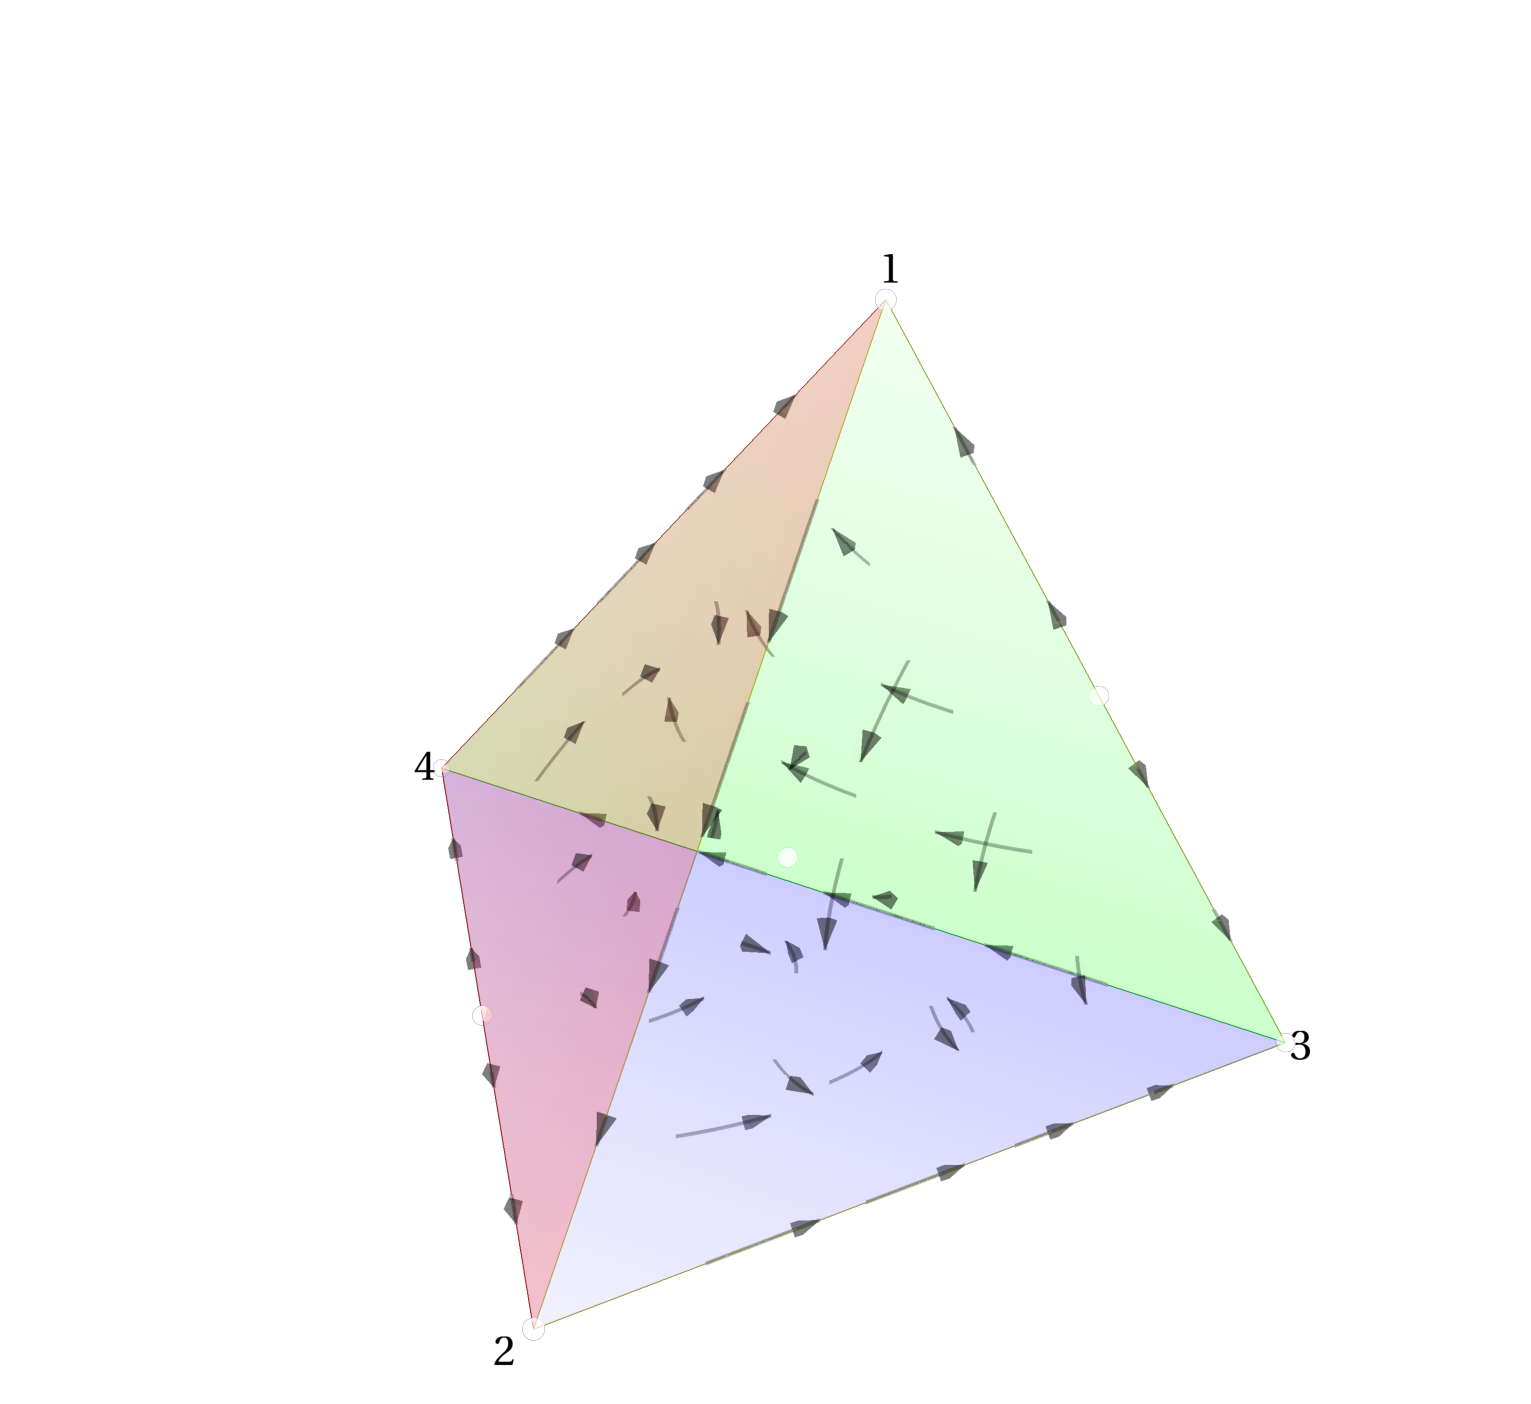
\includegraphics[width = 0.7\textwidth]{stable.pdf}
        \end{center}

        \item Case 2: The interior equilibrium is unstable.
        
        If $\mu<1$, then all the eigenvalues are positive and thus the interior equilibrium is unstable. The following is the phase portrait when $\mu = 2$.
        \begin{center}
                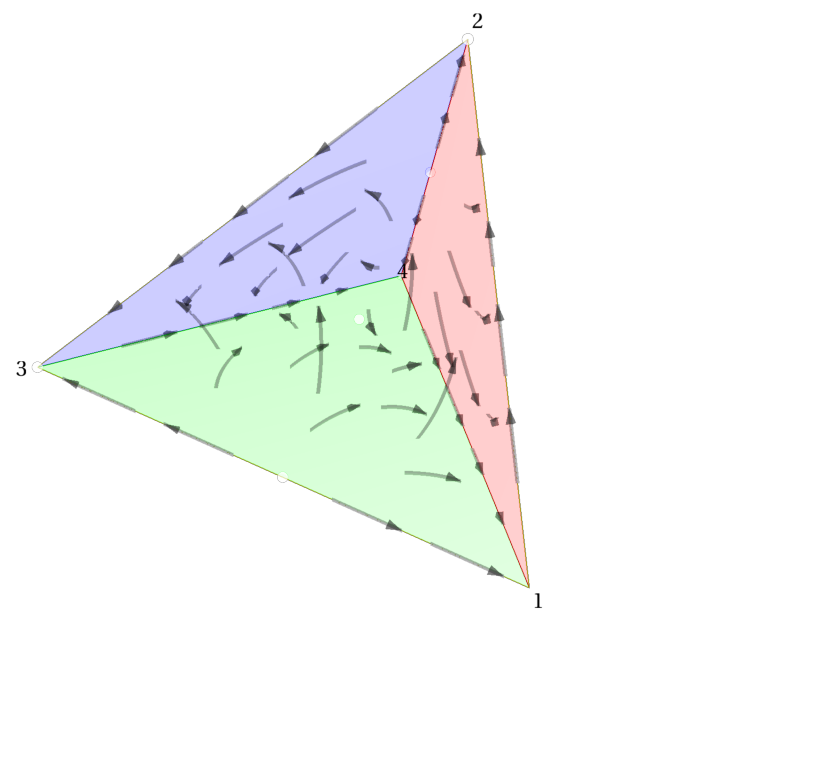
\includegraphics[width = 0.7\textwidth]{unstable.pdf}
        \end{center}

        \item Case 3: There is a periodic attractor near th interior equilibrium.

\end{itemize}




\tb{Problem 2}

\tb{Solution: }
\tb{a)} From the payoff matrix, it can be seen that to defect is the strongly dominant strategy. Thus, it is always a best response to whatever strategy its neighbors choose. Any agent that is not controlled will switch its strategy to defect in the next stage. Hence, under the best response rule, to render the 7 agents to be cooperative asymptotically, all the 7 agents have to be controlled. 

\tb{b)} Riehl and Cao \cite{b4} proposed an algorithm to compute the minimum number of controlled agents to drive all the agents to desired strategy under the imitating rule. Here I follow their algorithm as follows:
\begin{center}
        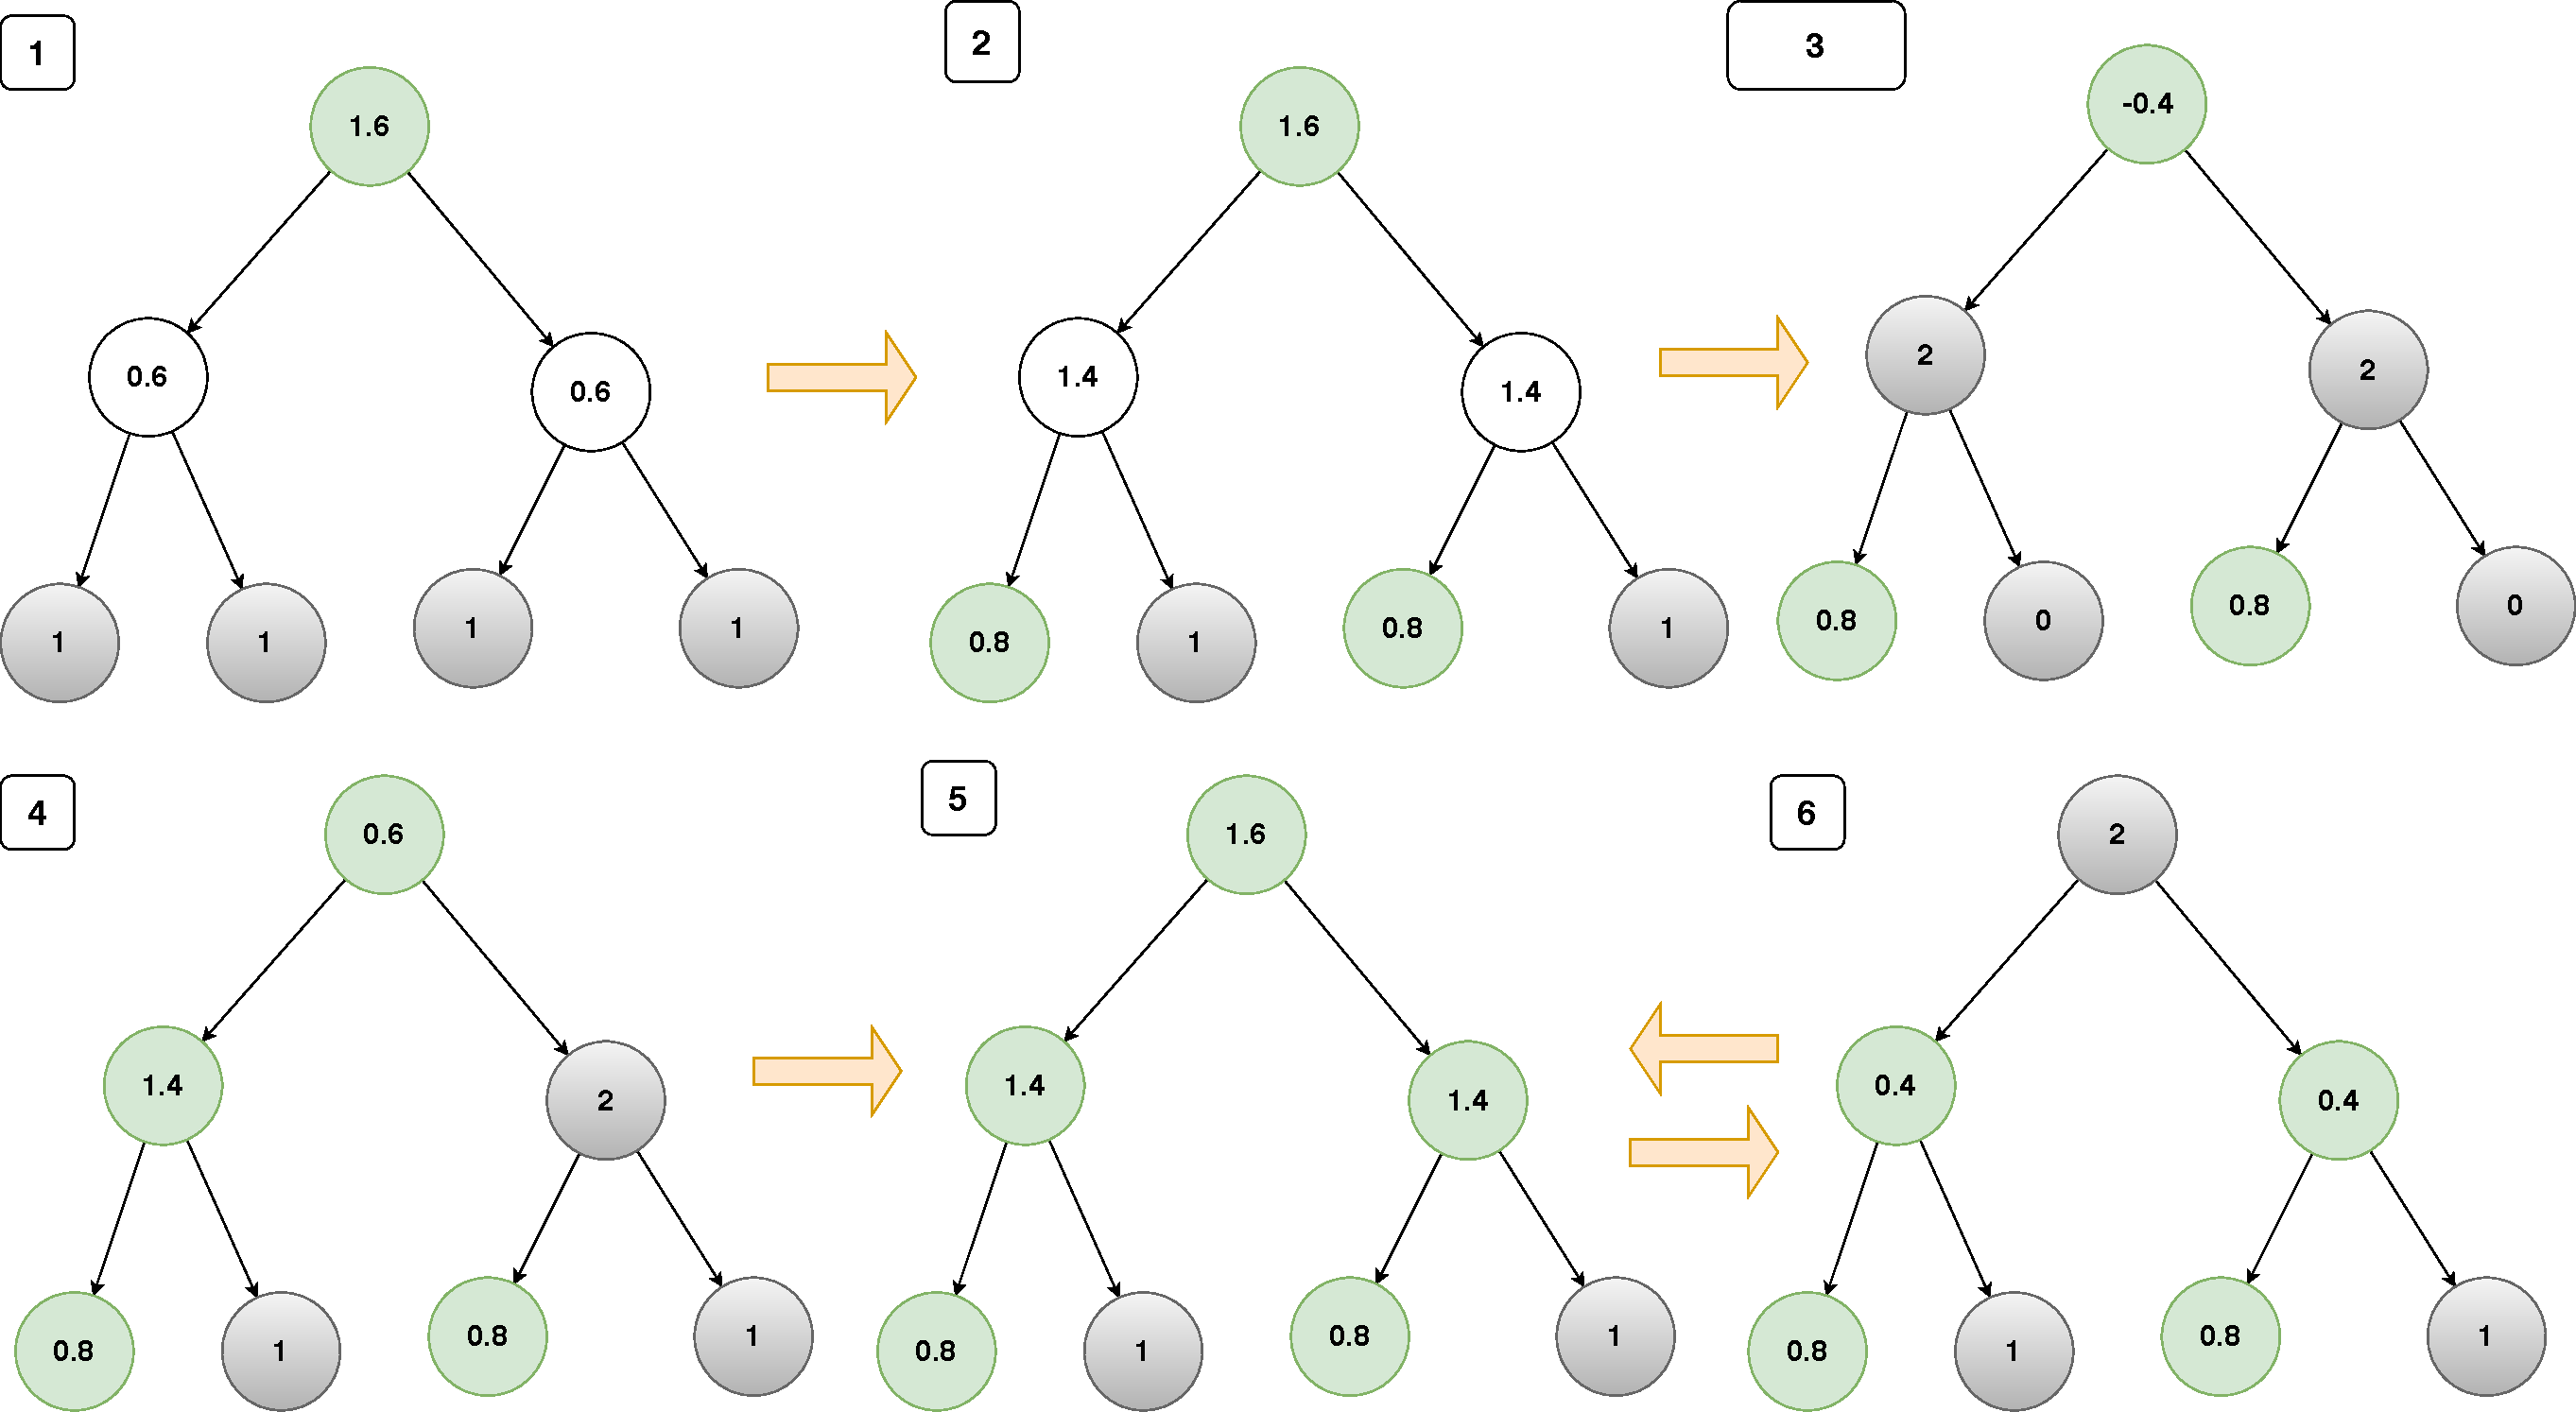
\includegraphics[width = 1.0\textwidth]{network_control.pdf}
\end{center}
where the green circles are agents being controlled, the white circles are agents to cooperative (playing strategy A) and the grey circles are agents to defect (playing strategy B). 

The steps are:
\begin{itemize}
        \item Assume the root agent is controlled and all other agents are playing A.
        \item From the bottom level, assuming each agent plays B and compute their payoff and their parents' payoff. 
        \item If any child's payoff is higher than its parents' payoff. Determine the minimum number and who should be controlled such that the parents' payoff is higher than the children. Repeat this for every sub-branch.
        \item Move to one upper level (second level in this case). Do the previous step again to determine the agents who should be controlled in this level.
        \item Repeat the previous two steps level by level until the root.
        \item Remove the root from the controlled agents set and check if the network can be driven to desired state. In this case the answer is not. So the root has to stay in the controlled agents set.
\end{itemize}

In conclude, by applying the algorithm, we can obtain that the minimum number of controlled agents is 6 and they are shown in the above figure.


\tb{Problem 3}

\tb{Solution:} To find the presented examples, I used Matlab to search and simulate the evolutionary process of networks, which is listed at the end of this solution. In all examples, a graph is given to represent a network, in which the green circular nodes are coordinating agents and the red rectangular nodes are anti-coordinating agents. All agents have two strategies to play, $A$ and $B$ and update their strategies synchronously.

\tb{a)} Yes. Here is an example:
\begin{center}
        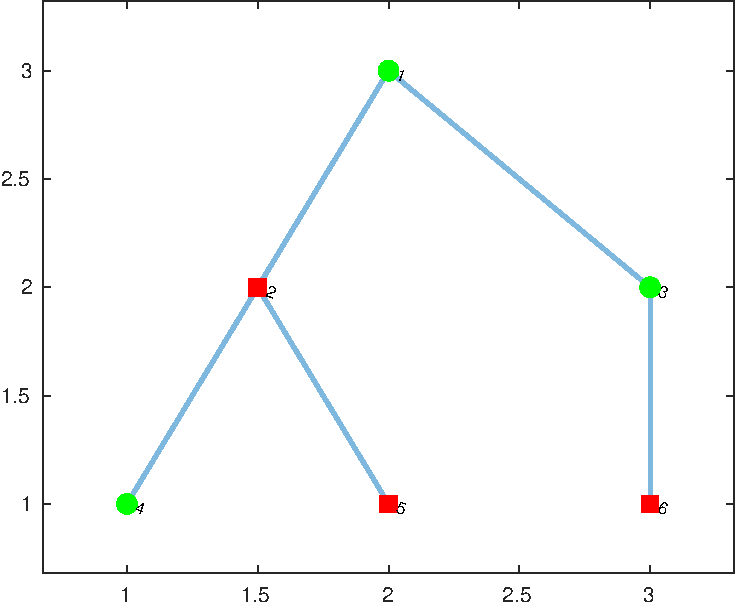
\includegraphics[width = 0.7\textwidth]{converge.pdf}
\end{center}
where 1,3,4 are coordinating agents and 2,5,6 are anti-coordinating agents and their initial playing strategies are $\{A,A,A,B,B,B\}$. The threshold is set to be $\tau_i = 0.5, i = 1,\dots,6$. For all agents, if $n_i^A(k)=\tau_i\tn{deg}_i$, they keep their current strategy, i.e. $z_i = x_i(k)$. According to the simulation, we can obtain the evolution of this network:
\begin{equation*}
        \begin{aligned}
                &\{A,A,A,B,B,B\} \\
                \ra &\{A,A,A,A,B,B\} \\ 
                \ra &\{A,B,A,A,B,B\} \\
                \ra &\{A,B,A,B,A,B\} \\
                \ra &\{\color{red}A,B,A,B,A,B\}
        \end{aligned}
\end{equation*}
Finally it converge to an equilibrium $\{A,B,A,B,A,B\}$.

\tb{b)} Yes. Here is an example:
\begin{center}
        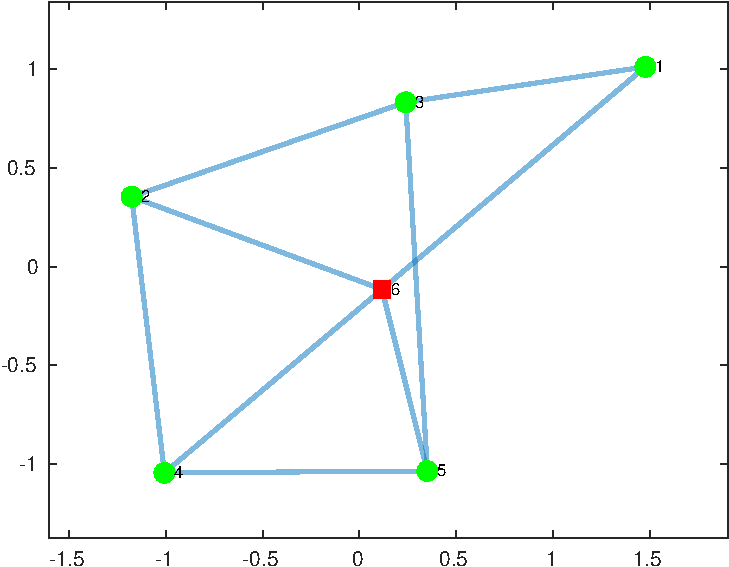
\includegraphics[width = 0.7\textwidth]{pd2.pdf}
\end{center}
where 1,2,3,4,5 are coordinating agents and 6 is an anti-coordinating agents and their initial playing strategies are $\{A,A,A,B,B,B\}$. The threshold is set to be $\tau = [ 0.3848,0.1626,\\0.7968,0.1138,0.1588,0.3558]^T$. For all agents, if $n_i^A(k)=\tau_i\tn{deg}_i$, they keep their current strategy, i.e. $z_i = x_i(k)$. According to the simulation, we can obtain the evolution of this network:
\begin{equation*}
        \begin{aligned}
                &\{A,A,A,B,B,B\} \\
                \ra &\{A,A,B,A,A,B\} \\ 
                \ra &\{B,A,A,A,A,B\} \\
                \ra &\{\color{red}A,A,B,A,A,B\} \\
                \ra &\{\color{red}B,A,A,A,A,B\}
        \end{aligned}
\end{equation*}
Finally it converges to a periodic solution of period 2: $\{A,A,B,A,A,B\}\ra\{B,A,A,A,A,B\}$.

\tb{c)} Yes. Here is an example:
\begin{center}
        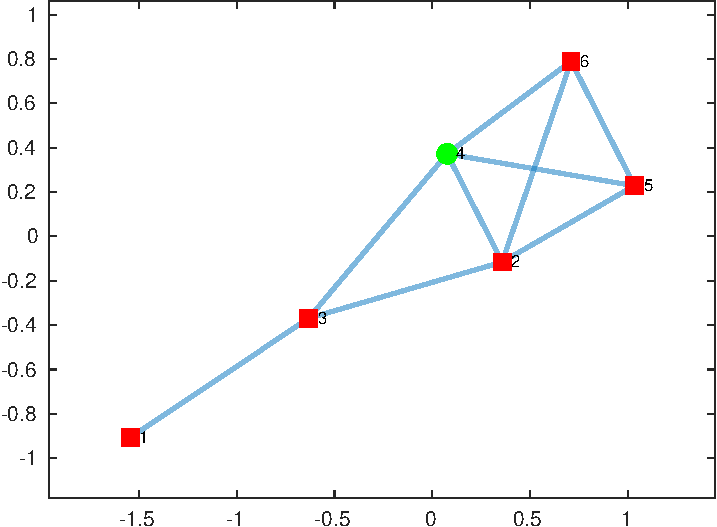
\includegraphics[width = 0.7\textwidth]{pd3.pdf}
\end{center}
where 4 is a coordinating agents and 1,2,3,5,6 are anti-coordinating agents and their initial playing strategies are $\{A,A,A,B,B,B\}$. The threshold is set to be $\tau_i = 0.8532, i = 1,\dots,6$. For all agents, if $n_i^A(k)=\tau_i\tn{deg}_i$, they keep their current strategy, i.e. $z_i = x_i(k)$. According to the simulation, we can obtain the evolution of this network:
\begin{equation*}
        \begin{aligned}
                &\{A,A,A,B,B,B\} \\
                \ra &\{B,A,A,B,A,A\} \\ 
                \ra &\{B,A,A,A,A,A\} \\
                \ra &\{B,B,A,A,B,B\} \\
                \ra &\{\color{red}B,A,A,B,A,A\} \\
                \ra &\{\color{red}B,A,A,A,A,A\} \\
                \ra &\{\color{red}B,B,A,A,B,B\} \\
        \end{aligned}
\end{equation*}
Finally it converges to a periodic solution of period 2: $\{B,A,A,B,A,A\}\ra\{B,A,A,A,A,A\}\ra\{B,B,A,A,B,B\}$.

\tb{d)} No. First, I have searched for periodic solution of period 2, 3, 4, 5 and 6 and I can always find an example. This indicates that it is almost surely converges to an equilibrium or a periodic solution. However, this does not mean that there is no case in which it will not converge. Hence, a rigorous proof is needed to prove that it will always converge. Nevertheless, I have no idea how to give such a rigorous proof. But I can show the property in a naive way.

Given a network, denote $x(k) = \{x_i(k),i=1,\dots,6\}$ the state vector of the network at stage $k$ and $x(k)\in\X$, where $\X$ is the feasible set of $x$. Then it is apparent that $\X$ is finite. Thus, for any $x(k)$, we can always find such a stage in the future who has the same state as current stage, i.e.
\begin{equation*}
        \exists\lambda\in\N, ~~s.t. ~~x(k+\lambda) = x(k)
\end{equation*}
Thus, under the linear threshold model, the network will always converge to an equilibrium or a periodic solution with finite period.

\tb{Matlab Code for Simulation}
\lstinputlisting[
  style      = Matlab-editor,
  basicstyle = \mlttfamily,
]{W4P3_sim_random.m}


%% Bibliography
\bibliographystyle{plain}
\begin{thebibliography}{99}

        \bibitem{b1} M. Maschler, E. Solan, and S. Zamir. \ti{Game Theory.} Cambridge: Cambridge University Press, 2013.

        \bibitem{b2} Weibull, Jörgen W. \ti{Evolutionary Game Theory}. MIT Press, 1997.

        \bibitem{b3} W. H. Sandholm, E. Dokumaci, and F. Franchetti. \ti{Dynamo: Diagrams for Evolutionary Game Dynamics}. 2012. http://www.ssc.wisc.edu/~whs/dynamo.

        \bibitem{b4} Riehl, J. R., and Cao, M. Minimal-agent control of evolutionary games on tree networks. In The 21st International Symposium on Mathematical Theory of Networks and Systems (Vol. 148), 2014.

        \bibitem{b5} H.K. Khalil. \ti{Nonlinear systems}. Prentice Hall, Upper Saddle River, USA, third edition, 2002.

\end{thebibliography}


\end{document}
